\chapter{Evaluation}
\label{sec:eval}

We have implemented \toolName{} on top of the Counter tool \cite{oopsla20}.
We use {\em four} SMT solvers running in parallel for solving
SMT proof obligations discharged by our proof discharge algorithm:
{\tt z3-4.8.7}, {\tt z3-4.8.14} \cite{z3}, {\tt Yices2-45e38fc} \cite{yices}, and {\tt cvc4-1.7} \cite{cvc4solver}.
An unroll factor of {\em four} is used to handle loop unrolling in the C implementation.
We use a default value of {\em eight} for over- and under-approximation depths ($d_o$ and $d_u$).
The default value of our unrolling parameter $k$ (used for categorization of proof obligations) is {\em five}.
We use a value of {\em five} for $\eta$ (used by {\em StrongestInvCover()} during weakening of \recursiveRelation{} invariants).

\toolName{} requires the user to provide a \SpecL{} program $S$ (specification), a C implementation $C$,
and a file that contains their input-output specifications.
For each function pair, \toolName{} attempts to find equivalence between their CFGs \sprog{} and \cprog{}
under their respective \pre{} and \post{} (given as part of input-output specification).
An equivalence check requires the identification of lifting constructors to relate C
values to the ADT values in \SpecL{} through  \recursiveRelations{}.
Such relations may be required at the entry of both programs (i.e. in the precondition \pre{}),
in the middle of both programs (i.e., in the invariants at intermediate product-CFG nodes),
and at the exit of both programs (i.e., in the postcondition \post{}).
\pre{} and \post{} are user-specified, whereas the inductive invariants are
inferred automatically by our algorithm.
During invariant inference, \toolName{} derives the candidate lifting constructors
from the user-specified \pre{} and \post{}.
More sophisticated approaches to finding lifting constructors are left as future work.

\section{Experiments}
\label{sec:experiments}
We consider programs involving four distinct ADTs, namely,
\inv{\small T1} \type{String}, \inv{\small T2} \type{List}, \inv{\small T3} \type{Tree}
and \inv{\small T4} \type{Matrix}.
For each \SpecL{} program specification, we consider multiple
C implementations that differ in their (a) layout and representation of ADTs, and
(b) algorithmic strategies. For example, a \type{Matrix}, in C, may be laid out
in a two-dimensional array, a one-dimensional array using row or column major
layouts etc. On the other hand, an optimized implementation may choose manual vectorization
of an inner-most loop. Next, we consider each ADT in more detail. For each,
we discuss (a) its corresponding programs, (b) C memory layouts and their lifting
constructors, and (c) varying algorithmic strategies.

\begin{table}[H]
\begin{center}
\caption{\label{tab:LiftingConsStr}String lifting constructors and their definitions.}
\begin{footnotesize}
\begin{tabular}{|l|l|}
\hline
\multicolumn{1}{|c|}{\Tstrut \Bstrut\footnotesize \bf Lifting Constructor} & \multicolumn{1}{c|}{\Tstrut \Bstrut \footnotesize \bf Definition} \\
\hline
\hline
\multicolumn{2}{|c|}{\makecell[c]{\Tstrut \Bstrut \inv{T1} {\tt Str = SInvalid | SNil | SCons(ch:i8, tail:Str)}  \qquad  {\tt OptStr = NotFound | Found(str:Str)} }} \\
\hline
\lifted{str}{\mem{}}{u8[]}{p\ctype{i32}} & \makecell[l]{\Tstrut \sumIf{p=0_\type{i32}} \ \sumThen{\cons{SInvalid}} \\
                                                        \Tstrut \sumElif{\arrIndex{p}{0_\type{i32}}{\mem{}}{i8}=0_\type{i8}} \ \sumThen{\cons{SNil}} \\
                                                \Tstrut \Bstrut \sumElse{\cons{SCons}(\arrIndex{p}{0_\type{i32}}{\mem{}}{i8}, \lifted{str}{\mem{}}{u8[]}{p+1_\type{i32}})}} \\
\hdashline[0.5px/3px]
\lifted{optstr}{\mem{}}{u8[]}{p\ctype{i32}} & \makecell[l]{\Tstrut \Bstrut \sumIf{p=0_\type{i32}} \ \sumThen{\cons{NotFound}} \sumElse{\cons{Found}(\lifted{str}{\mem{}}{u8[]}{p})}} \\
\hline
\lifted{str}{\mem{}}{lnode(u8)}{p\ctype{i32}} & \makecell[l]{\Tstrut \sumIf{p=0_\type{i32}} \ \sumThen{\cons{SInvalid}} \\
                                                             \Tstrut \sumElif{\structPointer{p}{\mem{}}{lnode}{val}=0_\type{i8}} \ \sumThen{\cons{SNil}} \\
                                                     \Tstrut \Bstrut \sumElse{\cons{SCons}(\structPointer{p}{\mem{}}{lnode}{val}, \lifted{str}{\mem{}}{lnode(u8)}{\structPointer{p}{\mem{}}{lnode}{next}})}} \\
\hdashline[0.5px/3px]
\lifted{optstr}{\mem{}}{lnode(u8)}{p\ctype{i32}} & \makecell[l]{\Tstrut \Bstrut \sumIf{p=0_\type{i32}} \ \sumThen{\cons{NotFound}} \sumElse{\cons{Found}(\lifted{str}{\mem{}}{lnode(u8)}{p})}} \\
\hline
\lifted{str}{\mem{}}{clnode(u8)}{p\ctype{i32},i\ctype{i2}} & \makecell[l]{\Tstrut \sumIf{p=0_\type{i32}} \ \sumThen{\cons{SInvalid}} \\
                                                                          \Tstrut \sumElif{\arrIndex{\structPointer{p}{\mem{}}{lnode}{chunk}}{i}{\mem{}}{i8}=0_\type{i8}} \ \sumThen{\cons{SNil}} \\
                                                                  \Tstrut \Bstrut \sumElse{\cons{SCons}(\arrIndex{\structPointer{p}{\mem{}}{lnode}{chunk}}{i}{\mem{}}{i8}, \lifted{str}{\mem{}}{clnode(u8)}{\ite{i=3_\type{i2}}{\structPointer{p}{\mem{}}{clnode}{next}}{p}, i+1_\type{i2}})}} \\
\hdashline[0.5px/3px]
\lifted{optstr}{\mem{}}{clnode(u8)}{p\ctype{i32},i\ctype{i2}} & \makecell[l]{\Tstrut \Bstrut \sumIf{p=0_\type{i32}} \ \sumThen{\cons{NotFound}} \sumElse{\cons{Found}(\lifted{str}{\mem{}}{clnode(u8)}{p,i})}} \\
\hline
\end{tabular}
\end{footnotesize}
\end{center}
\end{table}

\subsection{String}
\label{sec:expstring}
We wrote a single specification in \SpecL{} for each of the following
common string library functions: {\tt strlen}, {\tt strchr}, {\tt strcmp}, {\tt strspn},
{\tt strcspn}, and {\tt strpbrk}.  For each specification
program, we took multiple C implementations of that program, drawn from popular
libraries like {\tt glibc} \cite{glibc}, {\tt klibc} \cite{klibc}, {\tt newlib} \cite{newlib},
{\tt openbsd} \cite{openbsdlibc}, {\tt uClibc} \cite{uclibc},
{\tt dietlibc} \cite{dietlibc}, {\tt musl} \cite{musl}, and {\tt netbsd} \cite{netbsd}.
Some of these libraries implement the same function in two ways: one that is optimized
for code size and another that is optimized for runtime.
All these library implementations use a {\em null character} terminated array to represent
a string, and the
corresponding lifting constructor is \lift{str}{\mem{}}{u8[]}.
\type{u<N>} represents the N-bit unsigned integer type in C.
For example, \type{u8} represents \type{unsigned char} type.

Further, we implemented custom C programs for these functions that uses linked list
and {\em chunked linked list} data structures to represent a string.
In a chunked linked list, a single list node (linked through a {\tt next} pointer)
contains a small array (chunk) of values.
We use a default chunk size of four for our benchmarks.
The corresponding lifting constructors are \lift{str}{\mem{}}{lnode(u8)}
and \lift{str}{\mem{}}{clnode(u8)} respectively.
These lifting constructors are defined in \cref{tab:LiftingConsStr}.
\lift{str}{\mem{}}{lnode(u8)} requires a single
argument $p$ representing the pointer to the list node.
On the other hand, \lift{str}{\mem{}}{clnode(u8)} requires two arguments $p$
and $i$, where $p$ represents the pointer to the chunked linked list node
and $i$ represents the position of the initial character in the chunk.

\begin{figure}
\begin{tabular}{cc}
\begin{subfigure}[b]{0.55\textwidth}
\begin{center}
\begin{allLangEnvFoot}
~{\tiny \textcolor{mygray}{S0:}}~ OptStr strchr (Str s, i8 c) {
~{\tiny \textcolor{mygray}{S1:}}~   while ${\tt true}$:
~{\tiny \textcolor{mygray}{S2:}}~     assume ${\tt \neg (s\ is\ SInvalid)}$;
~{\tiny \textcolor{mygray}{S3:}}~     if s is SNil:
~{\tiny \textcolor{mygray}{S4:}}~       if c == ${\tt 0_{i8}}$: return Found(s);
~{\tiny \textcolor{mygray}{S5:}}~       return NotFound();
~{\tiny \textcolor{mygray}{S6:}}~     i8 ch $\coloneq$ s.char; // (s is SCons)
~{\tiny \textcolor{mygray}{S7:}}~     if c == ch: return Found(s);
~{\tiny \textcolor{mygray}{S8:}}~     s $\coloneq$ s.tail;
~{\tiny \textcolor{mygray}{SE:}}~ }
\end{allLangEnvFoot}
\end{center}
\caption{\label{fig:llStrchrSpecIR}Strchr Spec IR Program}
\end{subfigure}%
&
\begin{subfigure}[b]{0.46\textwidth}
\begin{center}
\begin{allLangEnvFoot}
~{\tiny \textcolor{mygray}{\ \ \ }}~ char* strchr(char* t, int c);
~{\tiny \textcolor{mygray}{}}~
~{\tiny \textcolor{mygray}{C0:}}~ i32 strchr (i32 t, i32 c) {
~{\tiny \textcolor{mygray}{C1:}}~   i8 ch $\coloneq$ ${\tt bvextract_{7:0}(c)}$
~{\tiny \textcolor{mygray}{C2:}}~   while $\mathrm{\tt t[0_{i32}]^m_{i8} \neq ch}$:
~{\tiny \textcolor{mygray}{C3:}}~     if $\mathrm{\tt t[0_{i32}]^m_{i8} == 0_{i8}}$:
~{\tiny \textcolor{mygray}{C4:}}~       return ${\tt 0_{i32}}$;
~{\tiny \textcolor{mygray}{C5:}}~     t $\coloneq$ t + ${\tt 1_{i32}}$
~{\tiny \textcolor{mygray}{C6:}}~   return t;
~{\tiny \textcolor{mygray}{CE:}}~ }
\end{allLangEnvFoot}
\end{center}
\caption{\label{fig:llStrchrCArrIR}Generic Strchr C IR Program using Array}
\end{subfigure}%
\\
\begin{subfigure}[b]{0.55\textwidth}
\begin{center}
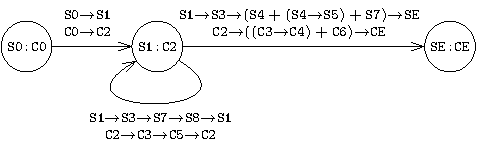
\includegraphics[scale=0.87]{chapters/figures/figStrchrProductCfg.pdf}
\end{center}
\caption{\label{fig:llStrchrProduct}XXX}
\end{subfigure}%
&
\begin{subfigure}[b]{0.50\textwidth}
\begin{center}
\begin{footnotesize}
\begin{tabular}{|c|l|}
\hline
\tt PC-Pair & \multicolumn{1}{c|} {\tt Invariants} \\
\hline
\hline
${\tt (S0:C0)}$ &
${\tt {\scriptsize \circled{P1}}\  s_{S}\indEq{}Cstr^{char[]}_{m}(t_{C})}$ \\ & ${\tt {\scriptsize \circled{P2}}\ c_{S}=bvextract_{7:0}(c_{C})}$ \\
\hline
${\tt (S1:C2)}$ &
${\tt {\scriptsize \circled{I1}}\  s_{S}\indEq{}Cstr^{char[]}_{m}(t_{C})}$ \\ & ${\tt {\scriptsize \circled{I2}}\  c_{S}=ch_{C}}$ \\
\hline
${\tt (SE:CE)}$ &
${\tt {\circled{E}}\  ret_{S}\indEq{}Cstr^{char[]}_{m}(ret_{C})}$ \\
\hline
\end{tabular}
\end{footnotesize}
\end{center}
\caption{\label{fig:llStrchrInvTable}XXX}
\end{subfigure}%
\\
\end{tabular}
\caption{\label{fig:llStrchr}XXX}
\end{figure}

\subsubsection{An Example : strchr}
\label{sec:strchrexample}
Additionally, we define an optional string type \type{OptStr} to specify
behaviour of functions that conditionally return a string (e.g., {\tt strchr}, {\tt strpbrk}).
The \type{OptStr} ADT along with its three lifting constructors for the three layouts of the \type{Str} ADT
are shown in \cref{tab:LiftingConsStr}.
{\tt strchr} accepts a string $t$ and a character $c$\footnote{TODO:Due to historical reasons, the type of $c$ is declared as \type{int}
to maintain backward compatibility with pre C-98 code.
However, the function is specified to cast it to a character and use it instead.} and returns
the longest substring of $t$ that begins with $c$, otherwise it returns a null pointer to indicate
failure to find $c$ in the string $t$.
In case $c$ is the null character, {\tt strchr} is defined to return the empty string ({\em not} the null value).
\Cref{fig:llStrchrSpecIR,fig:llStrchrCArrIR} shows the IRs of the {\tt strchr} \SpecL{} specification and
a generic C implementation respectively.
We demonstrate two important aspects of \toolName{} using this example -- (a) use of \sdef{} and \pre{} to restrict the C implementation
to only well-formed inputs (in \cref{sec:eqdef}),
and (b) need for correlating pathsets (instead of paths) (in \cref{sec:pathsetcorrel}).

Recall that a null-character terminated C string is only well-formed if the string itself does not belong to a region of memory containing the null pointer.
This wellformedness condition is necessary to prove that the pointer to the string returned in \cpc{6} (in \cref{fig:llStrchrCArrIR})
does not equal the null pointer (used uniquely to indicate a failure to find the character $c$ in the string $t$).
As previously discussed in \cref{sec:eqdef}, we expose this wellformedness condition in the specification using
the explicit \type{Str} data constructor \cons{SInvalid}.
Finally, we assert that \sv{s} in \cref{fig:llStrchrSpecIR} is wellformed using the {\tt assuming-do} statement
(\spc{3} in \cref{fig:llStrchrSpecIR}) and relate the non-null wellformedness condition of the C input string \cv{t}
with the condition of \sv{s} being \cons{SInvalid} using \pre{} (labeled \circled{\scriptsize P1} in \cref{fig:llStrchrInvs}).
Note the use of \lift{optstr}{\mem{}}{u8[]} in the postcondition (labeled \circled{E} in \cref{fig:llStrchrInvs}).

\Cref{fig:llStrchrProductCFG} shows the product-CFG showing the path correlations between \sprog{} and \cprog{}.
Consider the product-CFG edge \scedge{1}{2}{E}{E} correlating the pathsets:
$\pathset{S1,S3,(S4 \pathpar (\pathset{S4,S5}) \pathpar S7), SE}$ (in \sprog{}) and
$\pathset{C2,((\pathset{C3,C4}) \pathpar C6),CE}$ (in \cprog{}).
The $\rightarrow$ and $\pathpar$ operators are used to represent `series' and `parallel' path combinations.
The above two pathsets represent the following two sets
$\{ \spath{1,3,4,E},\spath{1,3,4,5,E},\spath{1,3,7,E} \}$ and
$\{ \cpath{2,3,4,E}, \cpath{2,6,E} \}$ respectively.
In \sprog{}, the case of \sv{c} being the null character is handled explicitly in \spc{4} while
\spc{7} handles the case where the string \sv{s} contains the (non-null) character \sv{c}.
However in \cprog{}, the above two cases are taken care of by the singular exit edge in \cpc{6}.
For a successful bisimulation proof, we are required to correlate the \cprog{} path
\cpath{2,6,E} with the \sprog{} pathset $\{ \spath{1,3,4,E}, \spath{1,3,7,E} \}$.
Such cases are rather frequent because the strongly-typed specification has to handle
each case explicitly while its C implementation may take advantage of the
underlying representation to generalize multiple explicit cases into one.

\begin{figure}
\begin{subfigure}[b]{0.5\textwidth}
\begin{center}
\begin{allLangEnvFoot}
~{\tiny \textcolor{mygray}{S0:}}~ i32 strlen (Str s) {
~{\tiny \textcolor{mygray}{S1:}}~   i32 len $\coloneqq$ ${\tt 0_{i32}}$;
~{\tiny \textcolor{mygray}{S2:}}~   while $\neg$(s is SNil):
~{\tiny \textcolor{mygray}{S3:}}~     assume $\neg$(s is SInvalid);
~{\tiny \textcolor{mygray}{S4:}}~     // (s is SCons)
~{\tiny \textcolor{mygray}{S5:}}~     s   $\coloneqq$ s.tail;
~{\tiny \textcolor{mygray}{S6:}}~     len $\coloneqq$ len + ${\tt 1_{i32}}$;
~{\tiny \textcolor{mygray}{S7:}}~   return len;
~{\tiny \textcolor{mygray}{SE:}}~ }
\end{allLangEnvFoot}
\end{center}
\caption{\label{fig:llStrlenSpecIR}Strlen specification}
\end{subfigure}%
\begin{subfigure}[b]{0.5\textwidth}
\begin{center}
\vspace{5px}
\begin{allLangEnvFoot}
~{\tiny \textcolor{mygray}{\ \ \ }}~ size_t strlen(char* s);

~{\tiny \textcolor{mygray}{C0:}}~ i32 strlen (i32 s) {
~{\tiny \textcolor{mygray}{C1:}}~   i32 i $\coloneqq$ ${\tt 0_{i32}}$;
~{\tiny \textcolor{mygray}{C2:}}~   while $\arrIndex{\tt s}{0_{i32}}{\mem{}}{i8} \neq 0_{i8}$:
~{\tiny \textcolor{mygray}{C3:}}~     s $\coloneqq$ s + ${\tt 1_{i32}}$;
~{\tiny \textcolor{mygray}{C4:}}~     i $\coloneqq$ i + ${\tt 1_{i32}}$;
~{\tiny \textcolor{mygray}{C5:}}~   return i;
~{\tiny \textcolor{mygray}{CE:}}~ }
\end{allLangEnvFoot}
\end{center}
\caption{\label{fig:llStrlenCArrIR}Generic strlen implementation using array}
\end{subfigure}
\begin{subfigure}[b]{1\textwidth}
\begin{center}
\begin{allLangEnvFoot}
~{\tiny \textcolor{mygray}{\ \ \ \ }}~ typedef struct clnode {
~{\tiny \textcolor{mygray}{\ \ \ \ }}~   char chunk[4]; struct clnode* next; } clnode;
~{\tiny \textcolor{mygray}{\ \ \ \ }}~ size_t strlen(clnode* cl);

~{\tiny \textcolor{mygray}{C0:\phantom{ }}}~ i32 strlen (i32 cl) {
~{\tiny \textcolor{mygray}{C1:\phantom{ }}}~   i32 hi $\coloneqq$ ${\tt 0x80808080_{i32}}$; i32 lo $\coloneqq$ ${\tt 0x01010101_{i32}}$;
~{\tiny \textcolor{mygray}{C2:\phantom{ }}}~   i32 i  $\coloneqq$ ${\tt 0_{i32}}$;
~{\tiny \textcolor{mygray}{C3:\phantom{ }}}~   while ${\tt true}$:
~{\tiny \textcolor{mygray}{C4:\phantom{ }}}~     i32 dword_ptr $\coloneqq$ addrof($\structPointer{\tt cl}{\mem{}}{clnode}{chunk}$);
~{\tiny \textcolor{mygray}{C5:\phantom{ }}}~     i32 dword     $\coloneqq$ $\arrIndex{\tt dword\_ptr}{0_{i32}}{\mem{}}{i32}$;
~{\tiny \textcolor{mygray}{C6:\phantom{ }}}~     if ${\tt ((dword - lo)\ \&\ (\sim dword)\ \&\ hi) \neq 0_{i32}}$:
~{\tiny \textcolor{mygray}{C7:\phantom{ }}}~       if $\arrIndex{\tt dword\_ptr}{0_{i32}}{\mem{}}{i8} = 0_{i8}$: return i;
~{\tiny \textcolor{mygray}{C8:\phantom{ }}}~       if $\arrIndex{\tt dword\_ptr}{1_{i32}}{\mem{}}{i8} = 0_{i8}$: return ${\tt i + 1_{i32}}$;
~{\tiny \textcolor{mygray}{C9:\phantom{ }}}~       if $\arrIndex{\tt dword\_ptr}{2_{i32}}{\mem{}}{i8} = 0_{i8}$: return ${\tt i + 2_{i32}}$;
~{\tiny \textcolor{mygray}{C10:}}~       if $\arrIndex{\tt dword\_ptr}{3_{i32}}{\mem{}}{i8} = 0_{i8}$: return ${\tt i + 3_{i32}}$;
~{\tiny \textcolor{mygray}{C11:}}~     cl $\coloneqq$ $\structPointer{\tt cl}{\mem{}}{clnode}{next}$; i  $\coloneqq$ ${\tt i + 4_{i32}}$;
~{\tiny \textcolor{mygray}{CE:\phantom{ }}}~ }
\end{allLangEnvFoot}
\end{center}
\caption{\label{fig:llStrlenCClistIR}Optimized strlen implementation using chunked linked list}
\end{subfigure}%
\caption{\label{fig:strlenSpecAndC}\Cref{fig:llStrlenSpecIR} shows the (abstracted) IR for the \SpecL{} specification of {\tt strlen}.
\Cref{fig:llStrlenCArrIR,fig:llStrlenCClistIR} show the (abstracted) IRs for two C implementations of {\tt strlen}.
\Cref{fig:llStrlenCArrIR} is a generic implementation using a nul-terminated array to represent a string, whereas
\cref{fig:llStrlenCClistIR} is an optimized implementation with a chunked linked list memory layout for a string.}
\end{figure}


\begin{figure}[t!]
\begin{tabular}{@{}c@{}c@{}}
\begin{subfigure}[b]{0.50\textwidth}
\begin{center}
{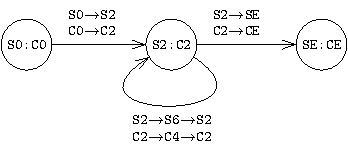
\includegraphics[scale=1.2]{chapters/figures/figStrlenArrProductCfg.pdf}}
\end{center}
\caption{\label{fig:StrlenArrProductCFG}Product-CFG for programs \cref{fig:llStrlenSpecIR,fig:llStrlenCArrIR}}
\end{subfigure}%
&
\begin{subfigure}[b]{0.50\textwidth}
\begin{center}
\begin{scriptsize}
\begin{tabular}{cl}
\toprule
{\bf PC-Pair} & \multicolumn{1}{c} {\bf Invariants} \\
\toprule
(\scpc{0}{0}) &
\Tstrut $\circled{P}\ \sv{s} \indEq{} \lifted{str}{\mem{}}{char[]}{\cv{s}}$ \\
\midrule
\multirow{2}{*}{(\scpc{2}{2})} &
\Tstrut $\circled{\tiny I1} \ \sv{s} \indEq{} \lifted{str}{\mem{}}{char[]}{\cv{s}}$ \\ &
\Tstrut $\circled{\tiny I2} \ \sv{len} = \cv{i}$ \\
\midrule
(\scpc{E}{E}) &
\Tstrut \Bstrut $\circled{E}\ \sv{ret} = \cv{ret}$ \\
\bottomrule
\end{tabular}
\end{scriptsize}
\end{center}
\caption{\label{fig:StrlenArrInvs}Invariants for product-CFG in \cref{fig:StrlenArrProductCFG}}
\end{subfigure}%
\\
\begin{subfigure}[b]{0.50\textwidth}
\begin{center}
{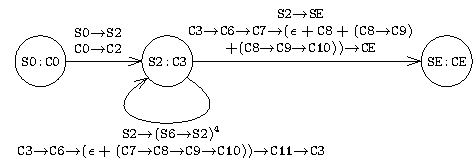
\includegraphics[scale=1.15]{chapters/figures/figStrlenClProductCfg.pdf}}
\end{center}
\caption{\label{fig:StrlenClProductCFG}Product-CFG for programs \cref{fig:llStrlenSpecIR,fig:llStrlenCClistIR}}
\end{subfigure}%
&
\begin{subfigure}[b]{0.50\textwidth}
\begin{center}
\begin{scriptsize}
\begin{tabular}{cl}
\toprule
{\bf PC-Pair} & \multicolumn{1}{c} {\bf Invariants} \\
\toprule
(\scpc{0}{0}) &
\Tstrut $\circled{P}\ \sv{s} \indEq{} \lifted{str}{\mem{}}{clnode}{\cv{cl},0}$ \\
\midrule
\multirow{2}{*}{(\scpc{2}{3})} &
\Tstrut $\circled{\tiny I1} \ \sv{s} \indEq{} \lifted{str}{\mem{}}{clnode}{\cv{cl},0}$ \\ &
\Tstrut $\circled{\tiny I2} \ \sv{len} = \cv{i}$ \\
\midrule
(\scpc{E}{E}) &
\Tstrut \Bstrut $\circled{E} \ \sv{ret} = \cv{ret}$ \\
\bottomrule
\end{tabular}
\end{scriptsize}
\end{center}
\caption{\label{fig:StrlenClInvs}Invariants for product-CFG in \cref{fig:StrlenClProductCFG}}
\end{subfigure}%
\end{tabular}
\caption{\label{fig:StrlenProductCFGsAndInvs}Product-CFGs and their node invariants representing bisimulation relations between the specification \cref{fig:llStrlenSpecIR}
and its two implementations in \cref{fig:llStrlenCArrIR,fig:llStrlenCClistIR} respectively.}
\end{figure}

\subsubsection{Another Example : strlen}
\Cref{fig:strlenSpecAndC} shows the {\tt strlen} specification and two vastly
different $C$ implementations. \Cref{fig:llStrlenCArrIR} is a generic implementation
using a null character terminated array to represent a string similar to a C-style string.
The second implementation in \cref{fig:llStrlenCClistIR} differs from \cref{fig:llStrlenCArrIR}
in the following: (a) it uses a chunked linked list data layout for the input string
and (b) it uses specialized bit manipulations to identify a null character in a chunk at a time.
\toolName{} is able to automatically find a bisimulation relation
for both implementations against the unaltered specification.
\Cref{fig:StrlenProductCFGsAndInvs} shows the product-CFG and invariants for each implementation.

Lifting constructors are named based on the C data layout being lifted
and the \SpecL{} ADT type of the lifted value.
For example, \lift{str}{}{u8[]} represents a \type{String} lifting constructor
for an array layout.
In general, we use the following naming convention for different C data layouts:
\type{T[]} represents an array of type \type{T} (e.g., \type{u8[]}).
\type{lnode(T)} represents a linked list node type containing a value of type \type{T}.
Similarly, \type{clnode(T)} and \type{tnode(T)} represent a chunked linked list and a tree node
with values of type \type{T} respectively.

\begin{table}[H]
\begin{center}
\caption{\label{tab:LiftingConsList}List lifting constructors and their definitions.}
\begin{footnotesize}
\begin{tabular}{|l|l|}
\hline
\multicolumn{1}{|c|}{\Tstrut \Bstrut \footnotesize \bf Lifting Constructor} & \multicolumn{1}{c|}{\Tstrut \Bstrut \footnotesize \bf Definition} \\
\hline
\hline
\multicolumn{2}{|c|}{\Tstrut \Bstrut \inv{T2} {\tt List = LNil | LCons(val:i32, tail:List)}} \\
\hline
\lifted{list}{\mem{}}{u32[]}{p\ i\ n\ctype{i32}} & \makecell[l]{\Tstrut \sumIf{i\geq_{u}n} \  \sumThen{\cons{LNil}} \\
                                                        \Tstrut \Bstrut \sumElse{\cons{LCons}(\arrIndex{p}{i}{\mem{}}{i32}, \lifted{list}{\mem{}}{u32[]}{p,i+1_\type{i32},n})}} \\
\hline
\lifted{list}{\mem{}}{lnode(u32)}{p\ctype{i32}} & \makecell[l]{\Tstrut \sumIf{p=0_\type{i32}} \  \sumThen{\cons{LNil}} \\
                                                       \Tstrut \Bstrut \sumElse{\cons{LCons}(\structPointer{p}{\mem{}}{lnode}{val}, \lifted{list}{\mem{}}{lnode}{\structPointer{p}{\mem{}}{lnode}{next}})}} \\
\hline
\lifted{list}{\mem{}}{clnode(u32)}{p\ctype{i32},i\ctype{i2}} & \makecell[l]{\Tstrut \sumIf{p=0_\type{i32}} \  \sumThen{\cons{LNil}} \\
                                                                    \Tstrut \Bstrut \sumElse{\cons{LCons}(\arrIndex{\structPointer{p}{\mem{}}{clnode}{chunk}}{i}{\mem{}}{i32}, \lifted{list}{\mem{}}{clnode}{\ite{i=3_\type{i2}}{\structPointer{p}{\mem{}}{clnode}{next}}{p},i+1_\type{i2}})}} \\
\hline
\end{tabular}
\end{footnotesize}
\end{center}
\end{table}

\subsection{List}
\label{sec:explist}
We wrote a \SpecL{} program specification that creates a list, a
program that traverses a list to compute the sum of its elements and a program
that computes the dot product of two lists. We use three different
data layouts for a list in C: array (\lift{list}{\mem{}}{u32[]}),
linked list (\lift{list}{\mem{}}{lnode(u32)}), and
a chunked linked list (\lift{list}{\mem{}}{clnode(u32)}).
The lifting constructors are shown in \cref{tab:LiftingConsList}.
Although similar to the String lifting constructors, these lifting
constructors differ widely in their data encoding. For example,
\lifted{list}{\mem{}}{u32[]}{p,i,n} represents a \type{List} value constructed
from a C array $p$ of size $n$ starting at the $i^{th}$ index. The list becomes empty
when we are at the end of the array. (\lift{list}{\mem{}}{lnode(u32)})
and (\lift{list}{\mem{}}{clnode(u32)}), on the other hand, encodes empty
lists (\cons{LNil}) using {\em null pointers}. These layouts are in contrast to the
\type{String} layouts, all of which uses a {\em null character} to
indicate the empty string.

% \begin{table}[H]
\begin{center}
\vspace{15px}
\caption{\label{tab:LiftingConsTree}Tree lifting constructors and their definitions}
\vspace{-15px}
\begin{scriptsize}
\relscale{1.17}
\begin{tabular}{|l|l|}
\hline
\multicolumn{1}{|c|}{\Tstrut \Bstrut\footnotesize \bf Lifting Constructor} & \multicolumn{1}{c|}{\Tstrut \Bstrut \footnotesize \bf Definition} \\
\hline
\hline
\multicolumn{2}{|c|}{\Tstrut \Bstrut \curvedtype{T3} {\tt Tree = TNil | TCons(val:i32, left:Tree, right:Tree)}} \\
\hline
\lifted{tree}{\mem{}}{u32[]}{p\ i\ n\ctype{i32}} & \makecell[l]{\Tstrut \sumIf{i \geq_u n} \  \sumThen{\cons{TNil}} \\
                                                        \Tstrut \Bstrut \sumElse{\cons{TCons}(\arrIndex{p}{i}{\mem{}}{i32}, \lifted{tree}{\mem{}}{u32[]}{p,2_\type{i32} \times i+1_\type{i32},n}, \lifted{tree}{\mem{}}{u32[]}{p,2_\type{i32} \times i+2_\type{i32},n})}} \\
\hline
\lifted{tree}{\mem{}}{tnode(u32)}{p\ctype{i32}} & \makecell[l]{\Tstrut \sumIf{p = 0_\type{i32}} \  \sumThen{\cons{TNil}} \\
                                                       \Tstrut \Bstrut \sumElse{\cons{TCons}(\structPointer{p\!}{\mem{}}{tnode}{\!\!val},\! \lifted{tree}{\mem{}}{tnode(u32)}{\structPointer{p\!}{\mem{}}{tnode}{\!\!left}},\! \lifted{tree}{\mem{}}{tnode(u32)}{\structPointer{p\!}{\mem{}}{tnode}{\!\!right}})}} \\
\hline
\end{tabular}
\end{scriptsize}
\end{center}
\end{table}

\subsection{Tree}
\label{sec:exptree}
We wrote a \SpecL{} program that sums all the nodes in a tree
through an inorder traversal using recursion. We use two different data layouts for a tree: 
(1) a flat array where a
{\em complete} binary tree is laid out in breadth-first search order commonly used for heaps (\lift{tree}{\mem{}}{u32[]}),
and (2) a linked tree node with two pointers for the left and right children (\lift{tree}{\mem{}}{tnode(u32)}) (shown in \cref{tab:LiftingConsTree}).
Both \SpecL{} and C programs contain non-tail recursive procedure calls for left and right children.
\toolName{} is able to correlate these recursive calls using user-provided \pre{} and \post{} as discussed in \cref{sec:correlfcalls}.
At the entry of the recursive calls, \toolName{} is required to prove that \pre{} holds for the arguments
and at the exit of the recursive calls, \toolName{} assumes \post{} on the returned states.

\begin{table}[t!]
\begin{center}
\caption{\label{tab:LiftingConsMatrix}Matrix and auxiliary List lifting constructors with their definitions}
\begin{scriptsize}
\relscale{1.25}
\begin{tabular}{|l|l|}
\hline
\multicolumn{1}{|c|}{\Tstrut \Bstrut \footnotesize \bf Lifting Constructor} & \multicolumn{1}{c|}{\Tstrut \Bstrut \footnotesize \bf Definition} \\
\hline
\hline
\multicolumn{2}{|c|}{\Tstrut \Bstrut \curvedtype{T4} {\tt Matrix = MNil | MCons(row:List, cols:Matrix)}} \\
\hline
\lifted{mat}{\mem{}}{u32[][]}{p\ i\ u\ v\ctype{i32}} & \makecell[l]{\Tstrut \sumIf{i \geq_u u} \  \sumThen{\cons{MNil}} \\
                                                            \Tstrut \Bstrut \sumElse{\cons{MCons}(\lifted{list}{\mem{}}{u32[]}{\arrIndex{p}{i}{\mem{}}{i32}, 0_\type{i32}, v}, \lifted{mat}{\mem{}}{u32[][]}{p, i+1_\type{i32}, u, v})}} \\
\hline
\lifted{list}{\mem{}}{u32[r]}{p\ i\ j\ u\ v\ctype{i32}} & \makecell[l]{\Tstrut \sumIf{j \geq_u v} \  \sumThen{\cons{LNil}} \\
                                                               \Tstrut \Bstrut \sumElse{\cons{LCons}(\arrIndex{p}{i \times v + j}{\mem{}}{i32}, \lifted{list}{\mem{}}{u32[r]}{p, i, j+1_\type{i32}, u, v})}} \\
\hdashline[0.5px/3px]
\lifted{mat}{\mem{}}{u32[r]}{p\ i\ u\ v\ctype{i32}} & \makecell[l]{\Tstrut \sumIf{i \geq_u u} \  \sumThen{\cons{MNil}} \\
                                                            \Tstrut \Bstrut \sumElse{\cons{MCons}(\lifted{list}{\mem{}}{u32[r]}{p,i,0_\type{i32},u,v}, \lifted{mat}{\mem{}}{u32[r]}{p, i+1_\type{i32}, u, v})}} \\
\hline
\lifted{list}{\mem{}}{u32[c]}{p\ i\ j\ u\ v\ctype{i32}} & \makecell[l]{\Tstrut \sumIf{j \geq_u v} \  \sumThen{\cons{LNil}} \\
                                                               \Tstrut \Bstrut \sumElse{\cons{LCons}(\arrIndex{p}{i + j \times u}{\mem{}}{i32}, \lifted{list}{\mem{}}{u32[c]}{p, i, j+1_\type{i32}, u, v})}} \\
\hdashline[0.5px/3px]
\lifted{mat}{\mem{}}{u32[c]}{p\ i\ u\ v\ctype{i32}} & \makecell[l]{\Tstrut \sumIf{i \geq_u u} \  \sumThen{\cons{MNil}} \\
                                                            \Tstrut \Bstrut \sumElse{\cons{MCons}(\lifted{list}{\mem{}}{u32[c]}{p,i,0_\type{i32},u,v}, \lifted{mat}{\mem{}}{u32[c]}{p, i+1_\type{i32}, u, v})}} \\
\hline
\lifted{mat}{\mem{}}{lnode(u32[])}{p\ v\ctype{i32}} & \makecell[l]{\Tstrut \sumIf{p = 0_\type{i32}} \sumThen{\cons{MNil}} \\
                                                           \Tstrut \Bstrut \sumElse{\cons{MCons}(\lifted{list}{\mem{}}{u32[]}{\structPointer{p}{\mem{}}{lnode}{val}, 0_\type{i32}, v}, \lifted{mat}{\mem{}}{lnode(u32[])}{\structPointer{p}{\mem{}}{lnode}{next},v})}} \\
\hline
\lifted{mat}{\mem{}}{lnode(u32)[]}{p\ i\ u\ctype{i32}} & \makecell[l]{\Tstrut \sumIf{i \geq_u u} \sumThen{\cons{MNil}} \\
                                                              \Tstrut \Bstrut \sumElse{\cons{MCons}(\lifted{list}{\mem{}}{lnode(u32)}{\arrIndex{p}{i}{\mem{}}{i32}}, \lifted{mat}{\mem{}}{lnode(u32)[]}{p,i+1_\type{i32},u})}} \\
\hline
\lifted{mat}{\mem{}}{clnode(u32)}{p\ i\ u\ctype{i32}} & \makecell[l]{\Tstrut \sumIf{i \geq_u u} \sumThen{\cons{MNil}} \\
                                                           \Tstrut \Bstrut \sumElse{\cons{MCons}(\lifted{list}{\mem{}}{clnode(u32)}{\arrIndex{p}{i}{\mem{}}{i32}, 0_\type{i2}}, \lifted{mat}{\mem{}}{clnode(u32)[]}{p,i+1_\type{i32},u})}} \\
\hline
\end{tabular}
\end{scriptsize}
\end{center}
\end{table}


\subsection{Matrix}
\label{sec:expmat}
We wrote a \SpecL{} program to count the frequency of a value appearing in a 2D matrix.
A matrix is represented as an ADT that resembles a \type{List} of \type{List}s (\inv{\small T4} in \cref{tab:LiftingConsMatrix}).
The C implementations for a \type{Matrix} object include
(a) a two-dimensional array (\lift{mat}{\mem{}}{u32[][]}), (b) a flattened row-major array (\lift{mat}{\mem{}}{u32[r]}),
(c) a flattened column-major array (\lift{mat}{\mem{}}{u32[c]}), (d) a linked list of 1D arrays (\lift{mat}{\mem{}}{lnode(u32[])}),
(e) a 1D array of linked lists (\lift{mat}{\mem{}}{lnode(u32)[]}) and (f) a 1D array of chunked linked list (\lift{mat}{\mem{}}{clnode(u32)[]})
data layouts. Note that both \type{T[r]} and \type{T[c]} represent a 1D array of type {\tt T}. The {\em r} and {\em c} simply
emphasizes that these arrays are used to represent matrices in row-major and column-major encodings respectively.
We also introduce two auxiliary lifting constructors, \lift{list}{\mem{}}{u32[r]} and \lift{list}{\mem{}}{u32[c]}
for lifting each row of matrices lifted using the corresponding \lift{mat}{\mem{}}{u32[r]} and \lift{mat}{\mem{}}{u32[c]} \type{Matrix} lifting
constructors. These constructors are listed in \cref{tab:LiftingConsMatrix}.

\begin{figure}[H]
\begin{scriptsize}
\begin{tabular}{lllclllc}
\toprule
{\bf Data Layout} & {\bf Variant} & {\bf Time(s)} & {\bf ${\tt \bf ( d_u, d_o )}$} & {\bf Data Layout} & {\bf Variant} & {\bf Time(s)} & {\bf ${\tt \bf ( d_u, d_o )}$} \\
\midrule
\multicolumn{4}{c}{\bf list} &                                              \multicolumn{4}{c}{\bf tree} \\
u32[] & sum naive & 16 & (1,2) &                                           u32[] & sum & 264 & (1,2) \\
      & sum opt & 49 & (4,5) &                                             tnode(u32) & sum & 204 & (1,2) \\
lnode(u32) & sum naive & 8 & (1,2) &                                      \multicolumn{4}{c}{\bf matfreq} \\             
           & sum opt & 54 & (4,5) &                                       char[][] & naive & 974 & (1,3) \\                                      
           & create & 426 & (1,1) &                                                & opt & 1.8k & (4,8) \\                                       
clnode(u32) & sum opt & 39 & (4,5) &                                      char[r] & naive & 958 & (1,3) \\                                       
\multicolumn{4}{c}{\bf strlen}   &                                            & opt & 1.9k & (4,8) \\                                        
char[] & dietlibc$\mathrm{_{small}}$ & 9 & (1,2) &                             char[c] & naive & 984 & (1,3) \\                                       
       & dietlibc$\mathrm{_{fast}}$ & 44 & (3,2) &                                     & opt & 1.9k & (4,6) \\
       & glibc & 52 & (3,2) &                                                  lnode(char[]) & naive & 753 & (1,3) \\
       & klibc & 9 & (1,2) &                                                         & opt & 1.7k & (4,6) \\ 
       & musl & 49 & (3,2) &                                                   lnode(char)[] & naive & 1.5k & (1,2) \\
       & netbsd & 9 & (1,2) &                                                                & opt & 2.3k & (4,6) \\
       & newlib & 50 & (3,2) &                                              clnode(char)[] & opt & 1.8k & (4,6) \\
       & openbsd & 8 & (1,2) &                                                \multicolumn{4}{c}{\bf strpbrk} \\ 
       & uClibc & 8 & (1,2) &                                                 char[], char[] & dietlibc & 398 & (1,2) \\
lnode(char) & naive & 13 & (1,2) &                                                          & opt      & 494 & (4,2) \\
            & opt & 49 & (3,5) &                                              char[], lnode(char) & naive & 392 & (1,2) \\
clnode(char) & opt & 45 & (3,5) &                                                                & opt & 540 & (4,2) \\ 
 \multicolumn{4}{c}{\bf strchr} &                                                 char[], clnode(char) & opt & 523 & (4,2) \\
char[] & dietlibc$\mathrm{_{small}}$ & 16 & (1,1) &                           lnode(char), char[] & naive & 497 & (1,2) \\
       & dietlibc$\mathrm{_{fast}}$ & 89 & (4,1) &                                               & opt & 602 & (4,2) \\ 
       & glibc & 127 & (4,1) &                                                lnode(char), lnode(char) & naive & 345 & (1,2) \\
       & klibc & 23 & (1,1) &                                                                           & opt & 503 & (4,2) \\
       & newlib$\mathrm{_{small}}$ & 15 & (1,1) &                         lnode(char), clnode(char) & opt & 572 & (4,2) \\
       & openbsd & 24 & (1,1) &                                             \multicolumn{4}{c}{\bf strcspn} \\
       & uClibc & 22 & (1,1) &                                              char[], char[] & dietlibc & 462 & (1,2) \\ 
lnode(char) & naive & 19 & (1,1) &                                                        & opt      & 538 & (4,2) \\ 
            & opt & 146 & (4,1) &                                           char[], lnode(char) & naive & 395 & (1,2) \\
\multicolumn{4}{c}{\bf strcmp}   &                                     & opt & 521 & (4,2) \\
char[], char[] & dietlibc$\mathrm{_{small}}$ & 39 & (1,1) &                 char[], clnode(char) & opt & 527 & (4,2) \\
       & freebsd & 39 & (1,1) &                                             lnode(char), char[] & naive & 601 & (1,2) \\
       & glibc & 41 & (1,1) &                                                                  & opt & 660 & (4,2) \\ 
       & klibc & 41 & (1,1) &                                               lnode(char), lnode(char) & naive & 349 & (1,2) \\
       & musl & 41 & (1,1) &                                                                        & opt & 502 & (4,2) \\
       & netbsd & 39 & (1,1) &                                              lnode(char), clnode(char) & opt & 595 & (4,2) \\
       & newlib$\mathrm{_{small}}$ & 42 & (1,1) &                              \multicolumn{4}{c}{\bf strspn} \\
       & newlib$\mathrm{_{fast}}$ & 405 & (4,1) &                              char[], char[] & dietlibc & 277 & (1,2)                   \\
       & openbsd & 40 & (1,1) &                                                              & opt      & 388 & (4,2)                    \\
       & uClibc & 38 & (1,1) &                                                 char[], lnode(char) & naive & 405 & (1,2)                 \\
lnode(char), lnode(char) & naive & 47 & (1,1) &                                                   & opt & 682 & (4,2)                    \\ 
            & opt & 293 & (4,1) &                                              char[], clnode(char) & opt & 535 & (4,2)                  \\
clnode(char), clnode(char) & opt & 254 & (4,1) &                               lnode(char), char[] & naive & 409 & (1,2)           \\
\multicolumn{4}{c}{\bf vecdot} &                                                          & opt & 553 & (4,2)              \\
u32[] & naive & 65 & (1,2) &                                                  lnode(char), lnode(char) & naive & 357 & (1,2)        \\
      & opt & 176 & (4,5)   &                                                                          & opt & 514 & (4,2)        \\
lnode(u32) & naive & 37 & (1,2) &                                              lnode(char), clnode(char) & opt & 616 & (4,2)         \\
           & opt & 120 & (4,5)   &                                               & & & \\
clnode(u32) & opt & 118 & (4,5)   &                                               & & & \\
\bottomrule
\end{tabular}
\end{scriptsize}
\vspace{-5px}
\caption{\label{tab:results}Equivalence checking times and minimum under- and over-approximation depth values at which equivalence checks succeeded.}
\vspace{-5px}
\end{figure}

\section{Results}
\label{sec:results}
\Cref{tab:results} lists the various C implementations and the time it took
to compute equivalence with their specifications. For functions that
take two or more data structures as arguments, we show
results for different combinations of data layouts for each argument.
We also show the minimum under-approximation ($d_u$) and over-approximation ($d_o$) depths
at which the equivalence proof completed (keeping all other parameters to their
default values).

During the verification of {\tt strchr} and {\tt strpbrk} implementations,
we identified an interesting subtlety. Since {\tt strchr} and {\tt strpbrk}
return null pointers to signify absence of the required character(s) in the input string,
we additionally need to model the UB assumption that the zero
address does not belong to the null character terminated array representing the string.
We use an explicit constructor \cons{SInvalid} to expose this well-formedness property in a \SpecL{} \type{String}.
Furthermore, we relate \cons{SInvalid} to the condition of C character pointer being null using the
lifting constructors \lifted{str}{\mem{}}{T}{p\ctype{i32},\dots} (as defined in \cref{tab:LiftingConsList}).
These lifting constructors are used as part of \pre{} to equate $S$ and $C$ input strings.
Finally in $S$, we model the absence of \cons{SInvalid} in the input string as a UB assumption using
the {\tt assuming-do} statement introduced in \cref{sec:speclang}.
Due to the \sdef{} assumption, this constraints the inputs to $S$ as well as $C$ to well-formed strings only.
This is an example where \sdef{} and \pre{} can be used to model wellformedness of values in $C$.

TODO: consider adding matrix data layouts (not programs) to illustrate the diversity of possible memory layouts being considered

\section{Limitations}
\label{sec:limitations}
\toolName{} is not without limitations.
Since \toolName{} is only interested in finding a bisimulation relation,
a whole class of non-bisimilar but equivalent program pairs is beyond our scope.
\toolName{} currently only supports bitvector affine and inequality relations, in addition to \recursiveRelations{}
based on the lifting constructors provided as part of \pre{} and \post{}.
Consequently, non-linear bitvector invariants (such as polynomial invariants) are not supported.
More importantly, \toolName{} does not attempt to infer lifting constructors and merely
uses the lifting constructors (with different arguments) provided as part of the input-output characteristics.
While our correlation and invariant inference algorithms are based on the Counter tool \cite{oopsla20}
designed primarily for translation validation between (C-like) unoptimized IR and assembly, we found them to be
quite effective for \SpecL{} to (C-like) IR as well.
However, \toolName{} inherits many of the limitations of the Counter tool.
For example, \toolName{} supports path specializations from \SpecL{} to C, but does not
search for path merging correlations.

In case of our proof discharge algorithm, we have identified a source of inefficiency for type II
proof obligations.
For a \recursiveRelation{} relating values of a non-linear ADT such as \type{Tree},
its $d$-depth approximation results in $\mathcal{O}(2^d)$ scalar equalities.
This is a source of major inefficiency due to generation of large SMT queries.
The completely of type III proof obligations is highly contingent on the precision
of our points-to analysis on \cprog{} as well as the deconstruction programs being
checked for equivanece as part of the nested bisimulation check.
We found our coarse-grained {\tt \{1,2+\}} categorization of allocation recency
combined with allocation-site based points-to analysis to be quite good at
identifying required points-to invariants.
However, such an abstraction is far from complete.